\documentclass[hyperref={pdfpagelabels=false}]{beamer}
\usepackage[ngerman]{babel}
\usepackage[utf8]{inputenc}


%\usepackage{lmodern}

\title{Thema 2.3: Apache Spark}   
\subtitle{Skalierbare verteilte Datenanalyse}
\author{Lukas Wappler} 
\date{\today} 

\usetheme{Malmoe}

\usepackage{beamerthemeshadow}


\useoutertheme{infolines}

%  \beamersetuncovermixins{\opaqueness<1>{25}}{\opaqueness<2->{15}}
%  sorgt dafuer das die Elemente die erst noch (zukuenftig) kommen 
%  nur schwach angedeutet erscheinen 
\beamersetuncovermixins{\opaqueness<1>{25}}{\opaqueness<2->{15}}
% klappt auch bei Tabellen, wenn teTeX verwendet wird\ldots



%NO FOOTLINE
%gets rid of bottom navigation bars
%\setbeamertemplate{footline}[frame number]{}

%gets rid of bottom navigation symbols
\setbeamertemplate{navigation symbols}{}

%gets rid of footer
%will override 'frame number' instruction above
%comment out to revert to previous/default definitions
\setbeamertemplate{footline}{}

\setbeamercovered{transparent}

%\setbeamertemplate{frametitle}{\nointerlineskip  
 %   \begin{beamercolorbox}[wd=\paperwidth,ht=2.75ex,dp=1.375ex]{frametitle}
  %      \hspace*{2ex}\insertframetitle \hfill {\insertframenumber} \hspace*{1ex}%
   % \end{beamercolorbox}}

%\addtobeamertemplate{headline}{}{\rule{\paperwidth}{3pt}}

\setbeamercolor{mycolor}{fg=blue,bg=blue}

\addtobeamertemplate{headline} 
{
  \leavevmode%
  \hbox{%
  \begin{beamercolorbox}[wd=.333333\paperwidth,ht=2.25ex,dp=1ex,center]{mycolor author in head/foot}%
    Lukas Wappler
		%\usebeamerfont{author in head/foot}\insertsection
  \end{beamercolorbox}%
  \begin{beamercolorbox}[wd=.333333\paperwidth,ht=2.25ex,dp=1ex,center]{mycolor title in head/foot}%
   
		Thema 2.3: Apache Spark		
  \end{beamercolorbox}%
  \begin{beamercolorbox}[wd=.333333\paperwidth,ht=2.25ex,dp=1ex,right]{mycolor date in head/foot}%
    \usebeamerfont{date in head/foot}\insertshortdate{}\hspace*{2em}
    \insertframenumber{} / \inserttotalframenumber \hspace*{2ex} 
  \end{beamercolorbox}}%
  \vskip0pt%
}


\begin{document}




\begin{frame}[plain,noframenumbering]
\titlepage
\end{frame} 


\begin{frame}
\frametitle{Inhaltsverzeichnis}
\setcounter{tocdepth}{1}
\tableofcontents
\end{frame} 





\section{} 
\begin{frame}
\frametitle{} 
\begin{center}
\textit{\LARGE{”Statistical thinking will one day be as necessary for efficient citizenship as the ability to read and write.“}}
\end{center}
\vspace{0.5cm} 
\begin{flushright}
\footnotesize{H.G. WELLS (1866-1946)\\ Science-Fiction-Roman-Autor\\ Der Krieg der Welten}
\end{flushright}

\end{frame}


\section*{Einleitung} 
\begin{frame}[t]
\frametitle{Einleitung} 

Heutige Probleme:
\begin{itemize}
\item  Immer mehr Daten 
\item  Datenanalysen werden immer schneller benötigt
\item  Systeme sind nicht skalierbar
\item  Großrechner sind teuer
\end{itemize}  


\visible<2-> { \huge{Ist Apache Spark die Lösung?}  }

\end{frame}

\section{Apache Spark} 
\begin{frame} [t]
\frametitle{Apache Spark} 


\begin{itemize}
	\item Cluster-System
	\item 2009 im AMPLab ins Leben gerufen
	\item 2010 Open Source	
	\item 2013 von der Apache Software Foundation übernommen
	\item 2014 Top Level Projekt		
\end{itemize}

\end{frame}

\section{Kern-Bibliotheken / Komponenten}
\begin{frame} [t]
\frametitle{Kern-Bibliotheken / Komponenten}


Nutzung der Komponenten
\begin{figure}[h]
  \centering
  \fbox{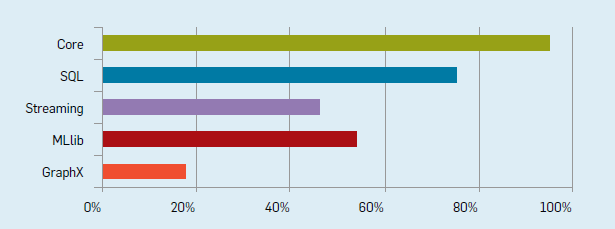
\includegraphics[width=110mm]{../../seminararbeit/bilder/spark_komponenten_nutzung.png}}	  
\end{figure}



\end{frame}

\subsubsection{Spark-Core}
\begin{frame} [t]
\frametitle{Spark-Core}

%\begin{itemize}
	%\item SparkContext
	%\item Cluster Manager
	%\item Worker Nodes		
%\end{itemize}

Aufbau \& Architektur

\begin{figure}[h]
  \centering
  \fbox{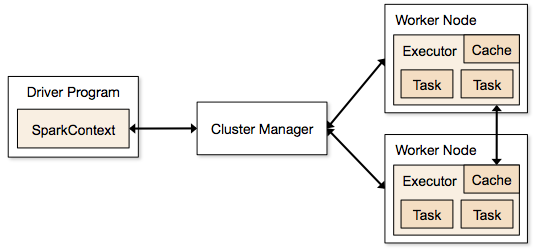
\includegraphics[width=80mm]{../../seminararbeit/bilder/cluster-overview.png}}
\end{figure}

\end{frame}

\subsubsection{RDD’s}
\begin{frame} [t]
\frametitle{RDD’s}

Resilient Distributed Datasets:
\begin{itemize}
	\item belastbar (fehlertolerant / ausfallsicher)
	\item verteilt (Daten sind in Blöcke unterteilt)
	\item nach Erstellung nur lesbar	
\end{itemize}

\vspace{0.4cm}

Operationen
\begin{itemize}
	\item Transformationen (filter, join, ...)
	\item Aktionen (reduce, count, ...)
\end{itemize}

\end{frame}


\subsection{SQL-Abfragen}
\subsubsection{Spark-SQL}
\begin{frame} [t]
\frametitle{Spark-SQL \& Dataframes}
\begin{itemize}
	\item eine Verbesserung von Shark
	\item kombiniert prozedurale Algorithmen \& relationale Datenbankabfragen
	\item neben RDD's werden auch DataFrames verwendet.	
	\item Anbindung unterschiedlichster Datenquellen:
		
		
		\begin{itemize}
			\item JSON
			\item JDBC
			\item Hive
			\item ...
		\end{itemize}
		
\end{itemize}



\end{frame}


\subsection{Verarbeitung von Datenströmen (Spark-Streaming)}
\begin{frame} [t]
\frametitle{Verarbeitung von Datenströmen (Spark-Streaming)}

\begin{itemize}
	\item RDD's werden zu DStreams erweitert
	\item Daten werden in einzelne Pakete unterteilt
	\item Transformationen können ausgeführt werden
\end{itemize}

\visible<2-> {
	\begin{figure}[h]
		\centering
		\fbox{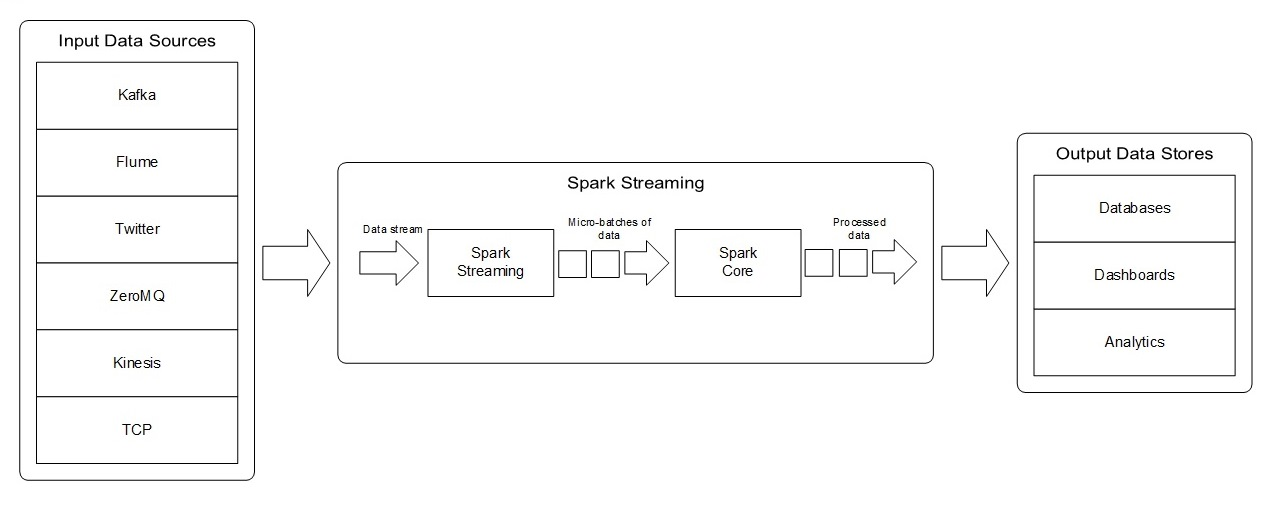
\includegraphics[width=110mm]{../../seminararbeit/bilder/spark_streaming.jpg}}
	\end{figure}
}
\end{frame}


\subsection{Berechnungen auf Graphen (GraphX)}
\begin{frame} [t]
\frametitle{Berechnungen auf Graphen (GraphX)}

\begin{itemize}
	\item Property-Graphen
	\item Abbildung der Graphen in RDD-Tupeln
	\item 1. RDD enthält Ecken
	\item 2. RDD enthält Kanten	
\end{itemize}

\visible<2-> {
	\begin{figure}[h]
		\centering
		\fbox{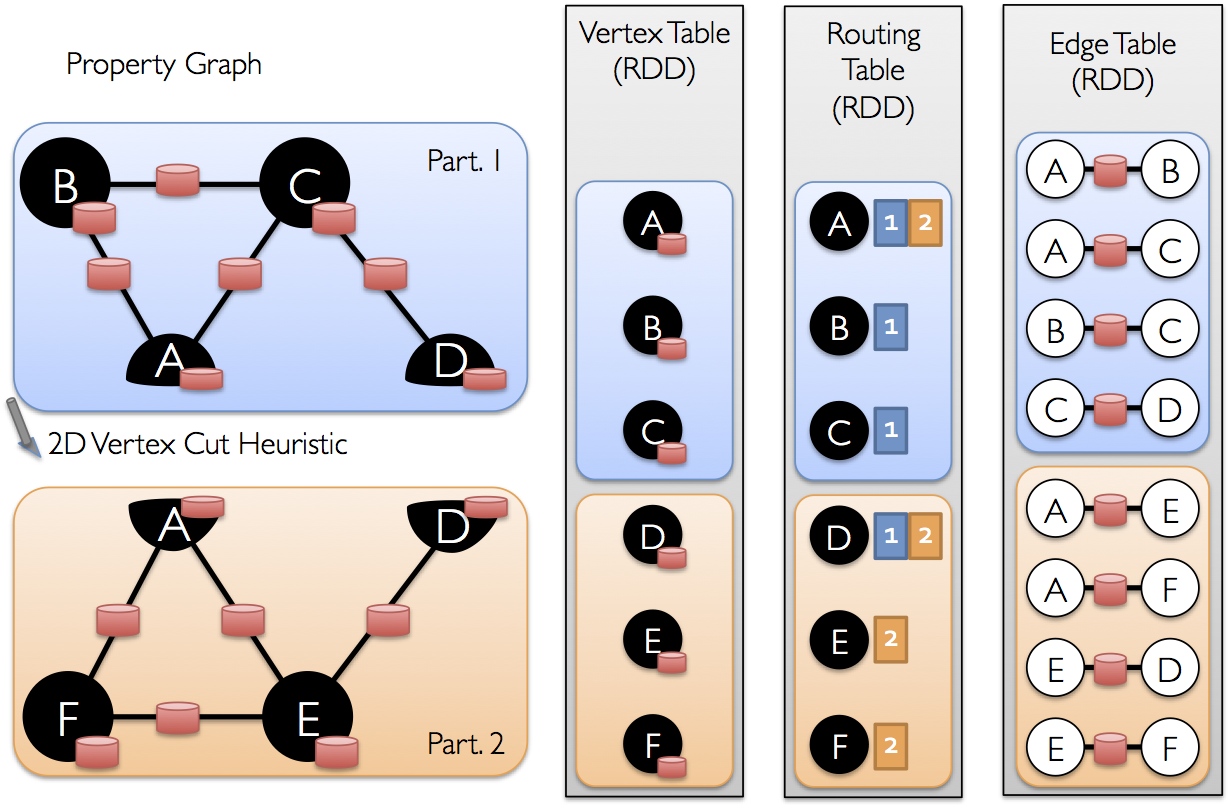
\includegraphics[width=80mm]{../../seminararbeit/bilder/vertex_routing_edge_tables.png}}
	\end{figure}
}

\end{frame}

\subsection{Maschinelles Lernen (MLlib)}
\begin{frame} [t]
\frametitle{Maschinelles Lernen (MLlib)}

\begin{itemize}
	\item Nutzt DataFrames
	\item Transformator (verändert die Daten)
	\item Estimator (Abstraktionen des Lernalgorithmus)
	\item Pipeline
\end{itemize}

\visible<2-> {
	\begin{figure}[h]
		\centering
		\fbox{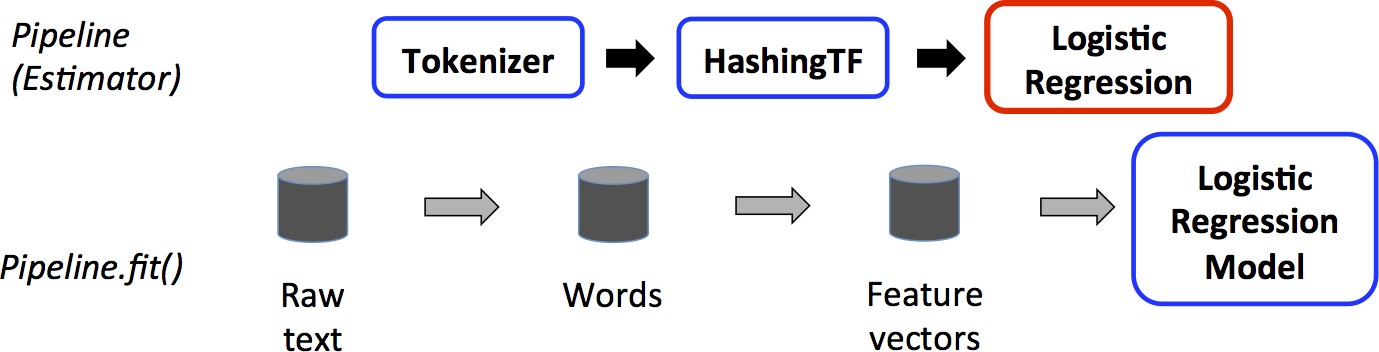
\includegraphics[width=110mm]{../../seminararbeit/bilder/ml-pipeline.png}}
	\end{figure}
}

\end{frame}

\subsection{Skalierung von R Programmen (SparkR)}
\begin{frame} [t]
\frametitle{Skalierung von R Programmen (SparkR)}

	Was ist R?
	\begin{itemize}		
		\item freie Programmiersprache
		\item statistische Berechnungen \& Grafiken				
		\item R läuft nur in einem Thread
	\end{itemize}
%\vspace{0.4cm}

Wie wird das Problem gelöst:
\begin{itemize}			
	\item R-JVM Brücke von R zu Java
	\item Kommunikation über Sockets 
\end{itemize}

\visible<2-> {
	\begin{figure}[h]
		\centering
		\fbox{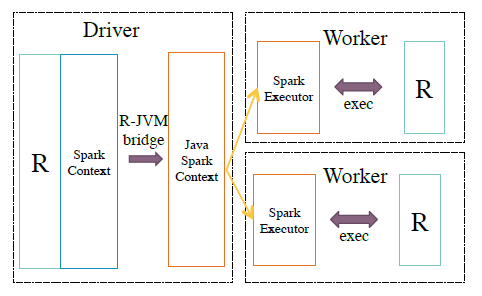
\includegraphics[width=60mm]{../../seminararbeit/bilder/spark_r_architecture.PNG}}
	\end{figure}
}

\end{frame}



\section{Demonstration}
\begin{frame} [t]
\frametitle{Demonstration}

Apache Spark im Einsatz \\
\textcolor[rgb]{0.75,0.75,0.75}{(Demo: Live oder Video.)}

\end{frame}


\begin{frame} [t]
\frametitle{Mehrere Komponenten im Verbund}

SparkCore, SparkSQL und MLlib im Verbund: 
\begin{itemize}	
	\item 100.000 Mitarbeiter Datensätze
	\item JSON-einlesen	
	\item Suchbegriffe trainieren
	\item Vorhersagen treffen
	\item Daten reduzieren	
	\item Sortieren
	\item Ausgabe der Ergebnisse	
\end{itemize}

\end{frame}


\section{Performance}
\begin{frame} [t]
\frametitle{Performance}

\begin{itemize}
	\item webbasierte Übersicht über Cluster
	\item schwer zu messen
	\item Fehler sind schwer zu lokalisieren
	\item Seiteneffekte bei verteilten Operationen	
\end{itemize}

\end{frame}

 \subsection{Besonderheiten bei der Speichernutzung}
\begin{frame} [t]
\frametitle{Besonderheiten bei der Speichernutzung}

\begin{itemize}
	\item Nutzung des Arbeitsspeichers
	\item speicherplatzeffiziente Datenstrukturen
	\item komprimierte Daten können Blockgrößen überschreiten	
\end{itemize}

\end{frame}

 \subsection{Netzwerk und I/O-Traffic}
\begin{frame} [t]
\frametitle{Netzwerk und I/O-Traffic}
Analysen mit:
\begin{itemize}
	\item 8.000 Nodes
	\item 1PB Daten	
\end{itemize}

\vspace{0.4cm}
\visible<2-> {
Optimierungen:
\begin{itemize}
	\item Daten von Festplatte zum Socket direkt kopieren
	\item Speichertabellen außerhalb des Java Heaps verwalten
	\item parallele Verarbeitung über mehrere Verbindungen	
\end{itemize}
}
\end{frame}


\section{Nutzung und Verbreitung}
\begin{frame} [t]
\frametitle{Nutzung und Verbreitung}

\begin{itemize}
	\item Skala, Python, Java, (R)
	\item viele Datenquellen
	\item viele Dateiformate	
	\item über 400 Mitwirkende (git contributors)
	\item aus über 100 Unternehmen
	\item Konferenzen (Spark Summit)
	\item 12,779 Sterne (Github)
\end{itemize}

\visible<2-> {
	\begin{figure}[h]
		\centering
		\fbox{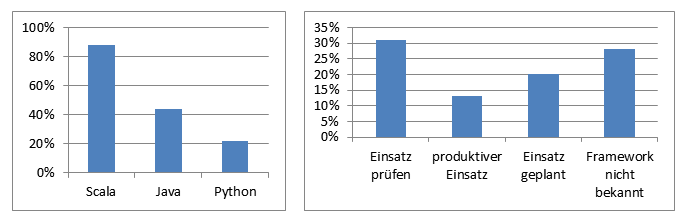
\includegraphics[width=100mm]{../../seminararbeit/excel/Nutzung.png}}
	\end{figure}
}

\end{frame}


\section{Fazit}
\begin{frame}[t]
\frametitle{}


\begin{columns}[t]
\begin{column}{5cm}
	
	Vorteile: \\
	
	\begin{itemize}
		\item vielfältig einsetzbar
		\item kann mit Speziallösungen mithalten
		\item gute Dokumentation \& Literatur	
		\item kostengünstig
		\item flexibel
	\end{itemize}
\end{column}
\begin{column}{5cm}

	Nachteile: \\
	
	\begin{itemize}		
		\item Mischung verschiedener Datenstrukturen schwierig
		\item veraltete News, Blogs oder Foren-Beiträge		
	\end{itemize}

\end{column}
\end{columns}




\end{frame}

\section{Ausblick und Weiterentwicklung}
\begin{frame} [t]
\frametitle{Ausblick und Weiterentwicklung}

\begin{itemize}
	\item Code ist über Github verfügbar
	\item ständige Weiterentwicklung
	\item jeder kann daran mitarbeiten
	\item 51 Releases (bzw. RC's)
	\item über 19.000 commits
	\item immer wieder Performancesteigerungen
\end{itemize}

\end{frame}


\section*{Vielen Dank}

\begin{frame} 
\frametitle{Vielen Dank}

\begin{center}
\Huge{Vielen Dank für Ihre Aufmerksamkeit!}
\end{center}

\end{frame}




\end{document}